\documentclass[1p]{elsarticle_modified}
%\bibliographystyle{elsarticle-num}

%\usepackage[colorlinks]{hyperref}
%\usepackage{abbrmath_seonhwa} %\Abb, \Ascr, \Acal ,\Abf, \Afrak
\usepackage{amsfonts}
\usepackage{amssymb}
\usepackage{amsmath}
\usepackage{amsthm}
\usepackage{scalefnt}
\usepackage{amsbsy}
\usepackage{kotex}
\usepackage{caption}
\usepackage{subfig}
\usepackage{color}
\usepackage{graphicx}
\usepackage{xcolor} %% white, black, red, green, blue, cyan, magenta, yellow
\usepackage{float}
\usepackage{setspace}
\usepackage{hyperref}

\usepackage{tikz}
\usetikzlibrary{arrows}

\usepackage{multirow}
\usepackage{array} % fixed length table
\usepackage{hhline}

%%%%%%%%%%%%%%%%%%%%%
\makeatletter
\renewcommand*\env@matrix[1][\arraystretch]{%
	\edef\arraystretch{#1}%
	\hskip -\arraycolsep
	\let\@ifnextchar\new@ifnextchar
	\array{*\c@MaxMatrixCols c}}
\makeatother %https://tex.stackexchange.com/questions/14071/how-can-i-increase-the-line-spacing-in-a-matrix
%%%%%%%%%%%%%%%

\usepackage[normalem]{ulem}

\newcommand{\msout}[1]{\ifmmode\text{\sout{\ensuremath{#1}}}\else\sout{#1}\fi}
%SOURCE: \msout is \stkout macro in https://tex.stackexchange.com/questions/20609/strikeout-in-math-mode

\newcommand{\cancel}[1]{
	\ifmmode
	{\color{red}\msout{#1}}
	\else
	{\color{red}\sout{#1}}
	\fi
}

\newcommand{\add}[1]{
	{\color{blue}\uwave{#1}}
}

\newcommand{\replace}[2]{
	\ifmmode
	{\color{red}\msout{#1}}{\color{blue}\uwave{#2}}
	\else
	{\color{red}\sout{#1}}{\color{blue}\uwave{#2}}
	\fi
}

\newcommand{\Sol}{\mathcal{S}} %segment
\newcommand{\D}{D} %diagram
\newcommand{\A}{\mathcal{A}} %arc


%%%%%%%%%%%%%%%%%%%%%%%%%%%%%5 test

\def\sl{\operatorname{\textup{SL}}(2,\Cbb)}
\def\psl{\operatorname{\textup{PSL}}(2,\Cbb)}
\def\quan{\mkern 1mu \triangleright \mkern 1mu}

\theoremstyle{definition}
\newtheorem{thm}{Theorem}[section]
\newtheorem{prop}[thm]{Proposition}
\newtheorem{lem}[thm]{Lemma}
\newtheorem{ques}[thm]{Question}
\newtheorem{cor}[thm]{Corollary}
\newtheorem{defn}[thm]{Definition}
\newtheorem{exam}[thm]{Example}
\newtheorem{rmk}[thm]{Remark}
\newtheorem{alg}[thm]{Algorithm}

\newcommand{\I}{\sqrt{-1}}
\begin{document}

%\begin{frontmatter}
%
%\title{Boundary parabolic representations of knots up to 8 crossings}
%
%%% Group authors per affiliation:
%\author{Yunhi Cho} 
%\address{Department of Mathematics, University of Seoul, Seoul, Korea}
%\ead{yhcho@uos.ac.kr}
%
%
%\author{Seonhwa Kim} %\fnref{s_kim}}
%\address{Center for Geometry and Physics, Institute for Basic Science, Pohang, 37673, Korea}
%\ead{ryeona17@ibs.re.kr}
%
%\author{Hyuk Kim}
%\address{Department of Mathematical Sciences, Seoul National University, Seoul 08826, Korea}
%\ead{hyukkim@snu.ac.kr}
%
%\author{Seokbeom Yoon}
%\address{Department of Mathematical Sciences, Seoul National University, Seoul, 08826,  Korea}
%\ead{sbyoon15@snu.ac.kr}
%
%\begin{abstract}
%We find all boundary parabolic representation of knots up to 8 crossings.
%
%\end{abstract}
%\begin{keyword}
%    \MSC[2010] 57M25 
%\end{keyword}
%
%\end{frontmatter}

%\linenumbers
%\tableofcontents
%
\newcommand\colored[1]{\textcolor{white}{\rule[-0.35ex]{0.8em}{1.4ex}}\kern-0.8em\color{red} #1}%
%\newcommand\colored[1]{\textcolor{white}{ #1}\kern-2.17ex	\textcolor{white}{ #1}\kern-1.81ex	\textcolor{white}{ #1}\kern-2.15ex\color{red}#1	}

{\Large $\underline{12n_{0868}~(K12n_{0868})}$}

\setlength{\tabcolsep}{10pt}
\renewcommand{\arraystretch}{1.6}
\vspace{1cm}\begin{tabular}{m{100pt}>{\centering\arraybackslash}m{274pt}}
\multirow{5}{120pt}{
	\centering
	\includegraphics[width=112pt]{../../../GIT/diagram.site/Diagrams/png/2957_12n_0868.png}\\
\ \ \ A knot diagram\footnotemark}&
\allowdisplaybreaks
\textbf{Linearized knot diagam} \\
\cline{2-2}
 &
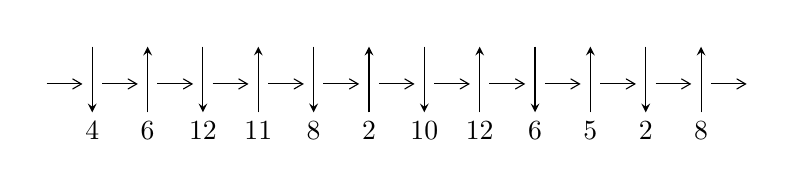
\begin{tikzpicture}[x=20pt, y=17pt]
	% nodes
	\node (C0) at (0, 0) {};
	\node (C1) at (1, 0) {};
	\node (C1U) at (1, +1) {};
	\node (C1D) at (1, -1) {4};

	\node (C2) at (2, 0) {};
	\node (C2U) at (2, +1) {};
	\node (C2D) at (2, -1) {6};

	\node (C3) at (3, 0) {};
	\node (C3U) at (3, +1) {};
	\node (C3D) at (3, -1) {12};

	\node (C4) at (4, 0) {};
	\node (C4U) at (4, +1) {};
	\node (C4D) at (4, -1) {11};

	\node (C5) at (5, 0) {};
	\node (C5U) at (5, +1) {};
	\node (C5D) at (5, -1) {8};

	\node (C6) at (6, 0) {};
	\node (C6U) at (6, +1) {};
	\node (C6D) at (6, -1) {2};

	\node (C7) at (7, 0) {};
	\node (C7U) at (7, +1) {};
	\node (C7D) at (7, -1) {10};

	\node (C8) at (8, 0) {};
	\node (C8U) at (8, +1) {};
	\node (C8D) at (8, -1) {12};

	\node (C9) at (9, 0) {};
	\node (C9U) at (9, +1) {};
	\node (C9D) at (9, -1) {6};

	\node (C10) at (10, 0) {};
	\node (C10U) at (10, +1) {};
	\node (C10D) at (10, -1) {5};

	\node (C11) at (11, 0) {};
	\node (C11U) at (11, +1) {};
	\node (C11D) at (11, -1) {2};

	\node (C12) at (12, 0) {};
	\node (C12U) at (12, +1) {};
	\node (C12D) at (12, -1) {8};
	\node (C13) at (13, 0) {};

	% arrows
	\draw[->,>={angle 60}]
	(C0) edge (C1) (C1) edge (C2) (C2) edge (C3) (C3) edge (C4) (C4) edge (C5) (C5) edge (C6) (C6) edge (C7) (C7) edge (C8) (C8) edge (C9) (C9) edge (C10) (C10) edge (C11) (C11) edge (C12) (C12) edge (C13) ;	\draw[->,>=stealth]
	(C1U) edge (C1D) (C2D) edge (C2U) (C3U) edge (C3D) (C4D) edge (C4U) (C5U) edge (C5D) (C6D) edge (C6U) (C7U) edge (C7D) (C8D) edge (C8U) (C9U) edge (C9D) (C10D) edge (C10U) (C11U) edge (C11D) (C12D) edge (C12U) ;
	\end{tikzpicture} \\
\hhline{~~} \\& 
\textbf{Solving Sequence} \\ \cline{2-2} 
 &
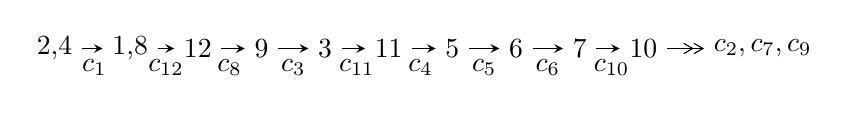
\begin{tikzpicture}[x=23pt, y=7pt]
	% node
	\node (A0) at (-1/8, 0) {2,4};
	\node (A1) at (17/16, 0) {1,8};
	\node (A2) at (17/8, 0) {12};
	\node (A3) at (25/8, 0) {9};
	\node (A4) at (33/8, 0) {3};
	\node (A5) at (41/8, 0) {11};
	\node (A6) at (49/8, 0) {5};
	\node (A7) at (57/8, 0) {6};
	\node (A8) at (65/8, 0) {7};
	\node (A9) at (73/8, 0) {10};
	\node (C1) at (1/2, -1) {$c_{1}$};
	\node (C2) at (13/8, -1) {$c_{12}$};
	\node (C3) at (21/8, -1) {$c_{8}$};
	\node (C4) at (29/8, -1) {$c_{3}$};
	\node (C5) at (37/8, -1) {$c_{11}$};
	\node (C6) at (45/8, -1) {$c_{4}$};
	\node (C7) at (53/8, -1) {$c_{5}$};
	\node (C8) at (61/8, -1) {$c_{6}$};
	\node (C9) at (69/8, -1) {$c_{10}$};
	\node (A10) at (11, 0) {$c_{2},c_{7},c_{9}$};

	% edge
	\draw[->,>=stealth]	
	(A0) edge (A1) (A1) edge (A2) (A2) edge (A3) (A3) edge (A4) (A4) edge (A5) (A5) edge (A6) (A6) edge (A7) (A7) edge (A8) (A8) edge (A9) ;
	\draw[->>,>={angle 60}]	
	(A9) edge (A10);
\end{tikzpicture} \\ 

\end{tabular} \\

\footnotetext{
The image of knot diagram is generated by the software ``\textbf{Draw programme}" developed by Andrew Bartholomew(\url{http://www.layer8.co.uk/maths/draw/index.htm\#Running-draw}), where we modified some parts for our purpose(\url{https://github.com/CATsTAILs/LinksPainter}).
}\phantom \\ \newline 
\centering \textbf{Ideals for irreducible components\footnotemark of $X_{\text{par}}$} 
 
\begin{align*}
I^u_{1}&=\langle 
63 u^7+216 u^6+255 u^5-250 u^4-354 u^3+222 u^2+419 b+903 u-430,\\
\phantom{I^u_{1}}&\phantom{= \langle  }-389 u^7-1633 u^6-2213 u^5-1815 u^4+11 u^3-2947 u^2+10475 a+2525 u-8904,\\
\phantom{I^u_{1}}&\phantom{= \langle  }u^8+2 u^7+2 u^6-5 u^5+u^4+3 u^3+15 u^2-14 u+5\rangle \\
I^u_{2}&=\langle 
-6 u^9+22 u^8-42 u^6+19 u^4-56 u^3-36 u^2+3 b-26 u-2,\\
\phantom{I^u_{2}}&\phantom{= \langle  }4 u^9-18 u^8+12 u^7+30 u^6-26 u^5-17 u^4+54 u^3-5 u^2+3 a-14 u-15,\\
\phantom{I^u_{2}}&\phantom{= \langle  }u^{10}-3 u^9-2 u^8+6 u^7+4 u^6-2 u^5+7 u^4+11 u^3+10 u^2+4 u+1\rangle \\
I^u_{3}&=\langle 
-9660231 u^{15}+63732863 u^{14}+\cdots+108707188 b+103207804,\\
\phantom{I^u_{3}}&\phantom{= \langle  }97383821 u^{15}-778749368 u^{14}+\cdots+108707188 a-952070632,\;u^{16}-8 u^{15}+\cdots-16 u+4\rangle \\
I^u_{4}&=\langle 
-3 u^3-15 u^2+2 b-33 u-26,\;9 u^3+35 u^2+28 a+67 u+34,\;u^4+7 u^3+23 u^2+38 u+28\rangle \\
I^u_{5}&=\langle 
- u^3- u^2+2 b-3 u,\;u^3-3 u^2+4 a+u-10,\;u^4+u^3+5 u^2+2 u+4\rangle \\
I^u_{6}&=\langle 
- u^7+6 u^6+u^5+20 u^4-3 u^3+10 u^2+56 b-2 u-24,\\
\phantom{I^u_{6}}&\phantom{= \langle  }2 u^7+2 u^6+5 u^5+16 u^4- u^3+36 u^2+14 a+11 u+20,\;u^8+5 u^6+2 u^5+9 u^4+8 u^3+12 u^2+8 u+4\rangle \\
I^u_{7}&=\langle 
u^2+b- u+1,\;a,\;u^4-2 u^3+2 u^2- u+1\rangle \\
I^u_{8}&=\langle 
4 u^3+9 u^2+11 b+u-15,\;-18 u^3-24 u^2+55 a-10 u+40,\;u^4-5 u+5\rangle \\
I^u_{9}&=\langle 
b- u,\;a+1,\;u^2+1\rangle \\
\\
\end{align*}
\raggedright * 9 irreducible components of $\dim_{\mathbb{C}}=0$, with total 60 representations.\\
\footnotetext{All coefficients of polynomials are rational numbers. But the coefficients are sometimes approximated in decimal forms when there is not enough margin.}
\newpage
\renewcommand{\arraystretch}{1}
\centering \section*{I. $I^u_{1}= \langle 63 u^7+216 u^6+\cdots+419 b-430,\;-389 u^7-1633 u^6+\cdots+10475 a-8904,\;u^8+2 u^7+\cdots-14 u+5 \rangle$}
\flushleft \textbf{(i) Arc colorings}\\
\begin{tabular}{m{7pt} m{180pt} m{7pt} m{180pt} }
\flushright $a_{2}=$&$\begin{pmatrix}1\\0\end{pmatrix}$ \\
\flushright $a_{4}=$&$\begin{pmatrix}0\\u\end{pmatrix}$ \\
\flushright $a_{1}=$&$\begin{pmatrix}1\\- u^2\end{pmatrix}$ \\
\flushright $a_{8}=$&$\begin{pmatrix}0.0371360 u^{7}+0.155895 u^{6}+\cdots-0.241050 u+0.850024\\-0.150358 u^{7}-0.515513 u^{6}+\cdots-2.15513 u+1.02625\end{pmatrix}$ \\
\flushright $a_{12}=$&$\begin{pmatrix}-0.101289 u^{7}-0.175847 u^{6}+\cdots-0.558473 u+1.33451\\- u\end{pmatrix}$ \\
\flushright $a_{9}=$&$\begin{pmatrix}0.0456325 u^{7}+0.0707399 u^{6}+\cdots-2.89260 u+1.80029\\-0.183771 u^{7}-0.630072 u^{6}+\cdots-0.300716 u+0.143198\end{pmatrix}$ \\
\flushright $a_{3}=$&$\begin{pmatrix}0.00507876 u^{7}-0.102587 u^{6}+\cdots+0.934129 u+0.406224\\-0.0381862 u^{7}+0.0119332 u^{6}+\cdots+0.119332 u+0.133652\end{pmatrix}$ \\
\flushright $a_{11}=$&$\begin{pmatrix}-0.101289 u^{7}-0.175847 u^{6}+\cdots-1.55847 u+1.33451\\- u\end{pmatrix}$ \\
\flushright $a_{5}=$&$\begin{pmatrix}-0.0712936 u^{7}-0.0787208 u^{6}+\cdots-0.827208 u+0.673527\\-0.0381862 u^{7}+0.0119332 u^{6}+\cdots+0.119332 u+0.133652\end{pmatrix}$ \\
\flushright $a_{6}=$&$\begin{pmatrix}-0.152916 u^{7}-0.215714 u^{6}+\cdots-2.19714 u+0.859208\\0.176611 u^{7}+0.319809 u^{6}+\cdots+1.19809 u-0.618138\end{pmatrix}$ \\
\flushright $a_{7}=$&$\begin{pmatrix}0.0236945 u^{7}+0.104095 u^{6}+\cdots-0.999045 u+0.241069\\0.176611 u^{7}+0.319809 u^{6}+\cdots+1.19809 u-0.618138\end{pmatrix}$ \\
\flushright $a_{10}=$&$\begin{pmatrix}-0.218219 u^{7}-0.375607 u^{6}+\cdots-2.30807 u+1.81497\\-0.0816229 u^{7}-0.136993 u^{6}+\cdots-1.36993 u+0.185680\end{pmatrix}$\\&\end{tabular}
\flushleft \textbf{(ii) Obstruction class $= -1$}\\~\\
\flushleft \textbf{(iii) Cusp Shapes $= \frac{61428}{52375} u^7+\frac{145366}{52375} u^6+\frac{182076}{52375} u^5-\frac{39694}{10475} u^4+\frac{38278}{52375} u^3+\frac{248544}{52375} u^2+\frac{32336}{2095} u-\frac{602992}{52375}$}\\~\\
\newpage\renewcommand{\arraystretch}{1}
\flushleft \textbf{(iv) u-Polynomials at the component}\newline \\
\begin{tabular}{m{50pt}|m{274pt}}
Crossings & \hspace{64pt}u-Polynomials at each crossing \\
\hline $$\begin{aligned}c_{1},c_{5},c_{7}\\c_{11}\end{aligned}$$&$\begin{aligned}
&u^8-2 u^7+2 u^6+5 u^5+u^4-3 u^3+15 u^2+14 u+5
\end{aligned}$\\
\hline $$\begin{aligned}c_{2},c_{6},c_{8}\\c_{12}\end{aligned}$$&$\begin{aligned}
&u^8- u^7-8 u^6+9 u^5+23 u^4-13 u^3+16 u^2-4 u+2
\end{aligned}$\\
\hline $$\begin{aligned}c_{3},c_{9}\end{aligned}$$&$\begin{aligned}
&5(5 u^8+29 u^7+\cdots+864 u+160)
\end{aligned}$\\
\hline $$\begin{aligned}c_{4},c_{10}\end{aligned}$$&$\begin{aligned}
&5(5 u^8+29 u^7+88 u^6+173 u^5+235 u^4+223 u^3+142 u^2+52 u+8)
\end{aligned}$\\
\hline
\end{tabular}\\~\\
\newpage\renewcommand{\arraystretch}{1}
\flushleft \textbf{(v) Riley Polynomials at the component}\newline \\
\begin{tabular}{m{50pt}|m{274pt}}
Crossings & \hspace{64pt}Riley Polynomials at each crossing \\
\hline $$\begin{aligned}c_{1},c_{5},c_{7}\\c_{11}\end{aligned}$$&$\begin{aligned}
&y^8+26 y^6-3 y^5+157 y^4-99 y^3+319 y^2-46 y+25
\end{aligned}$\\
\hline $$\begin{aligned}c_{2},c_{6},c_{8}\\c_{12}\end{aligned}$$&$\begin{aligned}
&y^8-17 y^7+128 y^6-443 y^5+503 y^4+607 y^3+244 y^2+48 y+4
\end{aligned}$\\
\hline $$\begin{aligned}c_{3},c_{9}\end{aligned}$$&$\begin{aligned}
&25(25 y^{8}+789 y^{7}+\cdots-150016 y+25600)
\end{aligned}$\\
\hline $$\begin{aligned}c_{4},c_{10}\end{aligned}$$&$\begin{aligned}
&25\\
&\cdot(25 y^8+39 y^7+60 y^6-83 y^5+123 y^4+427 y^3+732 y^2-432 y+64)
\end{aligned}$\\
\hline
\end{tabular}\\~\\
\newpage\flushleft \textbf{(vi) Complex Volumes and Cusp Shapes}
$$\begin{array}{c|c|c}  
\text{Solutions to }I^u_{1}& \I (\text{vol} + \sqrt{-1}CS) & \text{Cusp shape}\\
 \hline 
\begin{aligned}
u &= \phantom{-}1.025930 + 0.701004 I \\
a &= -0.761354 + 0.203728 I \\
b &= \phantom{-}0.93351 + 1.44138 I\end{aligned}
 & -4.59702 - 4.89276 I & -8.69831 + 5.22490 I \\ \hline\begin{aligned}
u &= \phantom{-}1.025930 - 0.701004 I \\
a &= -0.761354 - 0.203728 I \\
b &= \phantom{-}0.93351 - 1.44138 I\end{aligned}
 & -4.59702 + 4.89276 I & -8.69831 - 5.22490 I \\ \hline\begin{aligned}
u &= \phantom{-}0.422794 + 0.334865 I \\
a &= \phantom{-}0.741901 - 0.000101 I \\
b &= \phantom{-}0.013606 - 0.711717 I\end{aligned}
 & -0.740582 - 1.158680 I & -4.63203 + 6.37231 I \\ \hline\begin{aligned}
u &= \phantom{-}0.422794 - 0.334865 I \\
a &= \phantom{-}0.741901 + 0.000101 I \\
b &= \phantom{-}0.013606 + 0.711717 I\end{aligned}
 & -0.740582 + 1.158680 I & -4.63203 - 6.37231 I \\ \hline\begin{aligned}
u &= -0.96585 + 1.28563 I \\
a &= \phantom{-}1.086050 - 0.661498 I \\
b &= \phantom{-}0.30067 + 1.70085 I\end{aligned}
 & \phantom{-}13.8260 + 7.0293 I & \phantom{-}1.39449 - 3.33100 I \\ \hline\begin{aligned}
u &= -0.96585 - 1.28563 I \\
a &= \phantom{-}1.086050 + 0.661498 I \\
b &= \phantom{-}0.30067 - 1.70085 I\end{aligned}
 & \phantom{-}13.8260 - 7.0293 I & \phantom{-}1.39449 + 3.33100 I \\ \hline\begin{aligned}
u &= -1.48287 + 1.45144 I \\
a &= -0.746600 + 0.618962 I \\
b &= -0.24778 - 2.35508 I\end{aligned}
 & \phantom{-}11.2508 + 13.9556 I & -0.73615 - 5.79535 I \\ \hline\begin{aligned}
u &= -1.48287 - 1.45144 I \\
a &= -0.746600 - 0.618962 I \\
b &= -0.24778 + 2.35508 I\end{aligned}
 & \phantom{-}11.2508 - 13.9556 I & -0.73615 + 5.79535 I\\
 \hline 
 \end{array}$$\newpage\newpage\renewcommand{\arraystretch}{1}
\centering \section*{II. $I^u_{2}= \langle -6 u^9+22 u^8+\cdots+3 b-2,\;4 u^9-18 u^8+\cdots+3 a-15,\;u^{10}-3 u^9+\cdots+4 u+1 \rangle$}
\flushleft \textbf{(i) Arc colorings}\\
\begin{tabular}{m{7pt} m{180pt} m{7pt} m{180pt} }
\flushright $a_{2}=$&$\begin{pmatrix}1\\0\end{pmatrix}$ \\
\flushright $a_{4}=$&$\begin{pmatrix}0\\u\end{pmatrix}$ \\
\flushright $a_{1}=$&$\begin{pmatrix}1\\- u^2\end{pmatrix}$ \\
\flushright $a_{8}=$&$\begin{pmatrix}-\frac{4}{3} u^9+6 u^8+\cdots+\frac{14}{3} u+5\\2 u^9-\frac{22}{3} u^8+\cdots+\frac{26}{3} u+\frac{2}{3}\end{pmatrix}$ \\
\flushright $a_{12}=$&$\begin{pmatrix}u^9-3 u^8-2 u^7+6 u^6+4 u^5-2 u^4+7 u^3+11 u^2+10 u+4\\-3 u^9+\frac{26}{3} u^8+\cdots-\frac{70}{3} u-\frac{25}{3}\end{pmatrix}$ \\
\flushright $a_{9}=$&$\begin{pmatrix}-\frac{8}{3} u^9+\frac{26}{3} u^8+\cdots-11 u-\frac{7}{3}\\-\frac{10}{3} u^9+12 u^8+\cdots-\frac{61}{3} u^2-\frac{37}{3} u\end{pmatrix}$ \\
\flushright $a_{3}=$&$\begin{pmatrix}- u^9+3 u^8+2 u^7-6 u^6-4 u^5+2 u^4-7 u^3-11 u^2-10 u-4\\3 u^9-\frac{26}{3} u^8+\cdots+\frac{73}{3} u+\frac{25}{3}\end{pmatrix}$ \\
\flushright $a_{11}=$&$\begin{pmatrix}-2 u^9+\frac{17}{3} u^8+\cdots-\frac{40}{3} u-\frac{13}{3}\\-3 u^9+\frac{26}{3} u^8+\cdots-\frac{70}{3} u-\frac{25}{3}\end{pmatrix}$ \\
\flushright $a_{5}=$&$\begin{pmatrix}\frac{20}{3} u^9-22 u^8+\cdots+\frac{104}{3} u+7\\\frac{14}{3} u^9-\frac{49}{3} u^8+\cdots+\frac{67}{3} u+\frac{8}{3}\end{pmatrix}$ \\
\flushright $a_{6}=$&$\begin{pmatrix}6 u^9-\frac{62}{3} u^8+\cdots+\frac{82}{3} u+\frac{7}{3}\\-\frac{4}{3} u^9+\frac{16}{3} u^8+\cdots-2 u+\frac{4}{3}\end{pmatrix}$ \\
\flushright $a_{7}=$&$\begin{pmatrix}\frac{14}{3} u^9-\frac{46}{3} u^8+\cdots+\frac{76}{3} u+\frac{11}{3}\\-\frac{4}{3} u^9+\frac{16}{3} u^8+\cdots-2 u+\frac{4}{3}\end{pmatrix}$ \\
\flushright $a_{10}=$&$\begin{pmatrix}-8.66667 u^{9}+29.3333 u^{8}+\cdots-38.3333 u-4.66667\\-2 u^9+\frac{20}{3} u^8+\cdots-\frac{31}{3} u-\frac{4}{3}\end{pmatrix}$\\&\end{tabular}
\flushleft \textbf{(ii) Obstruction class $= -1$}\\~\\
\flushleft \textbf{(iii) Cusp Shapes $= -32 u^9+\frac{304}{3} u^8+52 u^7-220 u^6-92 u^5+\frac{364}{3} u^4-\frac{728}{3} u^3-324 u^2-\frac{620}{3} u-\frac{146}{3}$}\\~\\
\newpage\renewcommand{\arraystretch}{1}
\flushleft \textbf{(iv) u-Polynomials at the component}\newline \\
\begin{tabular}{m{50pt}|m{274pt}}
Crossings & \hspace{64pt}u-Polynomials at each crossing \\
\hline $$\begin{aligned}c_{1},c_{5},c_{7}\\c_{11}\end{aligned}$$&$\begin{aligned}
&u^{10}+3 u^9-2 u^8-6 u^7+4 u^6+2 u^5+7 u^4-11 u^3+10 u^2-4 u+1
\end{aligned}$\\
\hline $$\begin{aligned}c_{2},c_{6},c_{8}\\c_{12}\end{aligned}$$&$\begin{aligned}
&(u^5+u^4+2 u^3+u^2- u-1)^2
\end{aligned}$\\
\hline $$\begin{aligned}c_{3},c_{9}\end{aligned}$$&$\begin{aligned}
&(u-1)^{10}
\end{aligned}$\\
\hline $$\begin{aligned}c_{4},c_{10}\end{aligned}$$&$\begin{aligned}
&(u^5-3 u^4+6 u^3-7 u^2+5 u-3)^2
\end{aligned}$\\
\hline
\end{tabular}\\~\\
\newpage\renewcommand{\arraystretch}{1}
\flushleft \textbf{(v) Riley Polynomials at the component}\newline \\
\begin{tabular}{m{50pt}|m{274pt}}
Crossings & \hspace{64pt}Riley Polynomials at each crossing \\
\hline $$\begin{aligned}c_{1},c_{5},c_{7}\\c_{11}\end{aligned}$$&$\begin{aligned}
&y^{10}-13 y^9+\cdots+4 y+1
\end{aligned}$\\
\hline $$\begin{aligned}c_{2},c_{6},c_{8}\\c_{12}\end{aligned}$$&$\begin{aligned}
&(y^5+3 y^4-3 y^2+3 y-1)^2
\end{aligned}$\\
\hline $$\begin{aligned}c_{3},c_{9}\end{aligned}$$&$\begin{aligned}
&(y-1)^{10}
\end{aligned}$\\
\hline $$\begin{aligned}c_{4},c_{10}\end{aligned}$$&$\begin{aligned}
&(y^5+3 y^4+4 y^3-7 y^2-17 y-9)^2
\end{aligned}$\\
\hline
\end{tabular}\\~\\
\newpage\flushleft \textbf{(vi) Complex Volumes and Cusp Shapes}
$$\begin{array}{c|c|c}  
\text{Solutions to }I^u_{2}& \I (\text{vol} + \sqrt{-1}CS) & \text{Cusp shape}\\
 \hline 
\begin{aligned}
u &= -1.090900 + 0.471848 I \\
a &= \phantom{-}0.075129 - 0.502047 I \\
b &= -0.272955 + 0.216622 I\end{aligned}
 & -2.04480 + 6.94756 I & \phantom{-}1.39778 - 11.85170 I \\ \hline\begin{aligned}
u &= -1.090900 - 0.471848 I \\
a &= \phantom{-}0.075129 + 0.502047 I \\
b &= -0.272955 - 0.216622 I\end{aligned}
 & -2.04480 - 6.94756 I & \phantom{-}1.39778 + 11.85170 I \\ \hline\begin{aligned}
u &= \phantom{-}0.696642 + 0.968690 I \\
a &= \phantom{-}2.05550 + 0.04412 I \\
b &= \phantom{-}0.27367 - 2.40783 I\end{aligned}
 & -2.04480 - 6.94756 I & \phantom{-}1.39778 + 11.85170 I \\ \hline\begin{aligned}
u &= \phantom{-}0.696642 - 0.968690 I \\
a &= \phantom{-}2.05550 - 0.04412 I \\
b &= \phantom{-}0.27367 + 2.40783 I\end{aligned}
 & -2.04480 + 6.94756 I & \phantom{-}1.39778 - 11.85170 I \\ \hline\begin{aligned}
u &= -0.258396 + 0.483619 I \\
a &= -0.19552 + 2.23757 I \\
b &= \phantom{-}0.126970 + 0.325073 I\end{aligned}
 & \phantom{-}2.14309\phantom{ +0.000000I} & \phantom{-}10.96619 + 0. I\phantom{ +0.000000I} \\ \hline\begin{aligned}
u &= -0.258396 - 0.483619 I \\
a &= -0.19552 - 2.23757 I \\
b &= \phantom{-}0.126970 - 0.325073 I\end{aligned}
 & \phantom{-}2.14309\phantom{ +0.000000I} & \phantom{-}10.96619 + 0. I\phantom{ +0.000000I} \\ \hline\begin{aligned}
u &= -0.336196 + 0.392322 I \\
a &= \phantom{-}0.970972 - 0.269736 I \\
b &= -0.03146 + 1.71919 I\end{aligned}
 & -9.71882 + 0.63219 I & -5.88087 - 11.75603 I \\ \hline\begin{aligned}
u &= -0.336196 - 0.392322 I \\
a &= \phantom{-}0.970972 + 0.269736 I \\
b &= -0.03146 - 1.71919 I\end{aligned}
 & -9.71882 - 0.63219 I & -5.88087 + 11.75603 I \\ \hline\begin{aligned}
u &= \phantom{-}2.48885 + 0.02726 I \\
a &= \phantom{-}0.093920 + 0.941860 I \\
b &= -0.59622 - 4.37220 I\end{aligned}
 & -9.71882 + 0.63219 I & -5.88087 - 11.75603 I \\ \hline\begin{aligned}
u &= \phantom{-}2.48885 - 0.02726 I \\
a &= \phantom{-}0.093920 - 0.941860 I \\
b &= -0.59622 + 4.37220 I\end{aligned}
 & -9.71882 - 0.63219 I & -5.88087 + 11.75603 I\\
 \hline 
 \end{array}$$\newpage\newpage\renewcommand{\arraystretch}{1}
\centering \section*{III. $I^u_{3}= \langle -9.66\times10^{6} u^{15}+6.37\times10^{7} u^{14}+\cdots+1.09\times10^{8} b+1.03\times10^{8},\;9.74\times10^{7} u^{15}-7.79\times10^{8} u^{14}+\cdots+1.09\times10^{8} a-9.52\times10^{8},\;u^{16}-8 u^{15}+\cdots-16 u+4 \rangle$}
\flushleft \textbf{(i) Arc colorings}\\
\begin{tabular}{m{7pt} m{180pt} m{7pt} m{180pt} }
\flushright $a_{2}=$&$\begin{pmatrix}1\\0\end{pmatrix}$ \\
\flushright $a_{4}=$&$\begin{pmatrix}0\\u\end{pmatrix}$ \\
\flushright $a_{1}=$&$\begin{pmatrix}1\\- u^2\end{pmatrix}$ \\
\flushright $a_{8}=$&$\begin{pmatrix}-0.895836 u^{15}+7.16373 u^{14}+\cdots-21.1943 u+8.75812\\0.0888647 u^{15}-0.586280 u^{14}+\cdots+0.782914 u-0.949411\end{pmatrix}$ \\
\flushright $a_{12}=$&$\begin{pmatrix}-0.241595 u^{15}+2.01426 u^{14}+\cdots-6.73203 u+5.14019\\0.268938 u^{15}-1.87916 u^{14}+\cdots+2.75348 u-1.37285\end{pmatrix}$ \\
\flushright $a_{9}=$&$\begin{pmatrix}-0.380234 u^{15}+3.62129 u^{14}+\cdots-17.0765 u+9.18951\\0.105931 u^{15}-0.780917 u^{14}+\cdots+4.46533 u-2.37128\end{pmatrix}$ \\
\flushright $a_{3}=$&$\begin{pmatrix}-0.222657 u^{15}+2.13510 u^{14}+\cdots-10.9785 u+7.76734\\0.276444 u^{15}-1.95859 u^{14}+\cdots+3.06772 u-1.24414\end{pmatrix}$ \\
\flushright $a_{11}=$&$\begin{pmatrix}0.0273430 u^{15}+0.135102 u^{14}+\cdots-3.97855 u+3.76734\\0.268938 u^{15}-1.87916 u^{14}+\cdots+2.75348 u-1.37285\end{pmatrix}$ \\
\flushright $a_{5}=$&$\begin{pmatrix}-0.160445 u^{15}+1.90668 u^{14}+\cdots-11.6922 u+6.66721\\-0.214232 u^{15}+1.73017 u^{14}+\cdots-1.78134 u+0.144015\end{pmatrix}$ \\
\flushright $a_{6}=$&$\begin{pmatrix}-0.551916 u^{15}+4.80715 u^{14}+\cdots-14.5702 u+7.46698\\0.486247 u^{15}-4.00893 u^{14}+\cdots+11.7313 u-5.24454\end{pmatrix}$ \\
\flushright $a_{7}=$&$\begin{pmatrix}-0.0656690 u^{15}+0.798218 u^{14}+\cdots-2.83890 u+2.22243\\0.486247 u^{15}-4.00893 u^{14}+\cdots+11.7313 u-5.24454\end{pmatrix}$ \\
\flushright $a_{10}=$&$\begin{pmatrix}-0.967203 u^{15}+8.34540 u^{14}+\cdots-29.2669 u+13.9380\\0.00295473 u^{15}-0.352401 u^{14}+\cdots+5.57526 u-3.58334\end{pmatrix}$\\&\end{tabular}
\flushleft \textbf{(ii) Obstruction class $= 1$}\\~\\
\flushleft \textbf{(iii) Cusp Shapes $= -\frac{18550634}{27176797} u^{15}+\frac{155969047}{27176797} u^{14}+\cdots-\frac{461152304}{27176797} u+\frac{177121936}{27176797}$}\\~\\
\newpage\renewcommand{\arraystretch}{1}
\flushleft \textbf{(iv) u-Polynomials at the component}\newline \\
\begin{tabular}{m{50pt}|m{274pt}}
Crossings & \hspace{64pt}u-Polynomials at each crossing \\
\hline $$\begin{aligned}c_{1},c_{5},c_{7}\\c_{11}\end{aligned}$$&$\begin{aligned}
&u^{16}-8 u^{15}+\cdots-16 u+4
\end{aligned}$\\
\hline $$\begin{aligned}c_{2},c_{8}\end{aligned}$$&$\begin{aligned}
&(u^8+u^6-2 u^5-2 u^4+3 u^2+2 u+1)^2
\end{aligned}$\\
\hline $$\begin{aligned}c_{3},c_{9}\end{aligned}$$&$\begin{aligned}
&(u^8-4 u^6+2 u^5+7 u^4-6 u^3-4 u^2+6 u-1)^2
\end{aligned}$\\
\hline $$\begin{aligned}c_{4},c_{10}\end{aligned}$$&$\begin{aligned}
&(u^8+2 u^6+3 u^4-2 u^2-3)^2
\end{aligned}$\\
\hline $$\begin{aligned}c_{6},c_{12}\end{aligned}$$&$\begin{aligned}
&(u^8+u^6+2 u^5-2 u^4+3 u^2-2 u+1)^2
\end{aligned}$\\
\hline
\end{tabular}\\~\\
\newpage\renewcommand{\arraystretch}{1}
\flushleft \textbf{(v) Riley Polynomials at the component}\newline \\
\begin{tabular}{m{50pt}|m{274pt}}
Crossings & \hspace{64pt}Riley Polynomials at each crossing \\
\hline $$\begin{aligned}c_{1},c_{5},c_{7}\\c_{11}\end{aligned}$$&$\begin{aligned}
&y^{16}-16 y^{15}+\cdots-32 y+16
\end{aligned}$\\
\hline $$\begin{aligned}c_{2},c_{6},c_{8}\\c_{12}\end{aligned}$$&$\begin{aligned}
&(y^8+2 y^7-3 y^6-2 y^5+12 y^4-2 y^3+5 y^2+2 y+1)^2
\end{aligned}$\\
\hline $$\begin{aligned}c_{3},c_{9}\end{aligned}$$&$\begin{aligned}
&(y^8-8 y^7+30 y^6-68 y^5+103 y^4-108 y^3+74 y^2-28 y+1)^2
\end{aligned}$\\
\hline $$\begin{aligned}c_{4},c_{10}\end{aligned}$$&$\begin{aligned}
&(y^4+2 y^3+3 y^2-2 y-3)^4
\end{aligned}$\\
\hline
\end{tabular}\\~\\
\newpage\flushleft \textbf{(vi) Complex Volumes and Cusp Shapes}
$$\begin{array}{c|c|c}  
\text{Solutions to }I^u_{3}& \I (\text{vol} + \sqrt{-1}CS) & \text{Cusp shape}\\
 \hline 
\begin{aligned}
u &= -0.200065 + 0.849267 I \\
a &= -0.759797 + 0.858070 I \\
b &= -0.115947 + 0.816941 I\end{aligned}
 & \phantom{-}1.05416\phantom{ +0.000000I} & \phantom{-}                -6
1.330430 + 0. 10   I\phantom{ +0.000000I} \\ \hline\begin{aligned}
u &= -0.200065 - 0.849267 I \\
a &= -0.759797 - 0.858070 I \\
b &= -0.115947 - 0.816941 I\end{aligned}
 & \phantom{-}1.05416\phantom{ +0.000000I} & \phantom{-}                -6
1.330430 + 0. 10   I\phantom{ +0.000000I} \\ \hline\begin{aligned}
u &= \phantom{-}0.597550 + 0.533296 I \\
a &= -2.32458 - 0.98205 I \\
b &= -0.18223 + 2.10815 I\end{aligned}
 & -2.27209 - 5.91675 I & -0.74241 + 2.97163 I \\ \hline\begin{aligned}
u &= \phantom{-}0.597550 - 0.533296 I \\
a &= -2.32458 + 0.98205 I \\
b &= -0.18223 - 2.10815 I\end{aligned}
 & -2.27209 + 5.91675 I & -0.74241 - 2.97163 I \\ \hline\begin{aligned}
u &= \phantom{-}1.293270 + 0.159272 I \\
a &= -0.119407 + 0.360444 I \\
b &= -0.835722 - 0.165494 I\end{aligned}
 & -2.27209 - 5.91675 I & -0.74241 + 2.97163 I \\ \hline\begin{aligned}
u &= \phantom{-}1.293270 - 0.159272 I \\
a &= -0.119407 - 0.360444 I \\
b &= -0.835722 + 0.165494 I\end{aligned}
 & -2.27209 + 5.91675 I & -0.74241 - 2.97163 I \\ \hline\begin{aligned}
u &= -0.446252 + 0.506902 I \\
a &= -0.466779 + 0.410930 I \\
b &= \phantom{-0.000000 } -1.70507 I\end{aligned}
 & -9.66946\phantom{ +0.000000I} & -3.84561 + 0. I\phantom{ +0.000000I} \\ \hline\begin{aligned}
u &= -0.446252 - 0.506902 I \\
a &= -0.466779 - 0.410930 I \\
b &= \phantom{-0.000000 -}1.70507 I\end{aligned}
 & -9.66946\phantom{ +0.000000I} & -3.84561 + 0. I\phantom{ +0.000000I} \\ \hline\begin{aligned}
u &= \phantom{-}0.599542 + 0.283398 I \\
a &= \phantom{-}0.25980 - 1.48541 I \\
b &= \phantom{-}0.115947 + 0.816941 I\end{aligned}
 & \phantom{-}1.05416\phantom{ +0.000000I} & \phantom{-}                -6
1.330430 + 0. 10   I\phantom{ +0.000000I} \\ \hline\begin{aligned}
u &= \phantom{-}0.599542 - 0.283398 I \\
a &= \phantom{-}0.25980 + 1.48541 I \\
b &= \phantom{-}0.115947 - 0.816941 I\end{aligned}
 & \phantom{-}1.05416\phantom{ +0.000000I} & \phantom{-}                -6
1.330430 + 0. 10   I\phantom{ +0.000000I}\\
 \hline 
 \end{array}$$\newpage$$\begin{array}{c|c|c}  
\text{Solutions to }I^u_{3}& \I (\text{vol} + \sqrt{-1}CS) & \text{Cusp shape}\\
 \hline 
\begin{aligned}
u &= -1.197290 + 0.687330 I \\
a &= \phantom{-}0.028176 - 0.357279 I \\
b &= \phantom{-}0.835722 - 0.165494 I\end{aligned}
 & -2.27209 + 5.91675 I & -0.74241 - 2.97163 I \\ \hline\begin{aligned}
u &= -1.197290 - 0.687330 I \\
a &= \phantom{-}0.028176 + 0.357279 I \\
b &= \phantom{-}0.835722 + 0.165494 I\end{aligned}
 & -2.27209 - 5.91675 I & -0.74241 + 2.97163 I \\ \hline\begin{aligned}
u &= \phantom{-}0.823346 + 1.136370 I \\
a &= \phantom{-}1.41581 + 0.26433 I \\
b &= \phantom{-}0.18223 - 2.10815 I\end{aligned}
 & -2.27209 - 5.91675 I & -0.74241 + 2.97163 I \\ \hline\begin{aligned}
u &= \phantom{-}0.823346 - 1.136370 I \\
a &= \phantom{-}1.41581 - 0.26433 I \\
b &= \phantom{-}0.18223 + 2.10815 I\end{aligned}
 & -2.27209 + 5.91675 I & -0.74241 - 2.97163 I \\ \hline\begin{aligned}
u &= \phantom{-}2.52990 + 0.08941 I \\
a &= -0.033221 - 0.939974 I \\
b &= \phantom{-0.000000 -}4.50608 I\end{aligned}
 & -9.66946\phantom{ +0.000000I} & -3.84561 + 0. I\phantom{ +0.000000I} \\ \hline\begin{aligned}
u &= \phantom{-}2.52990 - 0.08941 I \\
a &= -0.033221 + 0.939974 I \\
b &= \phantom{-0.000000 } -4.50608 I\end{aligned}
 & -9.66946\phantom{ +0.000000I} & -3.84561 + 0. I\phantom{ +0.000000I}\\
 \hline 
 \end{array}$$\newpage\newpage\renewcommand{\arraystretch}{1}
\centering \section*{IV. $I^u_{4}= \langle -3 u^3-15 u^2+2 b-33 u-26,\;9 u^3+35 u^2+28 a+67 u+34,\;u^4+7 u^3+23 u^2+38 u+28 \rangle$}
\flushleft \textbf{(i) Arc colorings}\\
\begin{tabular}{m{7pt} m{180pt} m{7pt} m{180pt} }
\flushright $a_{2}=$&$\begin{pmatrix}1\\0\end{pmatrix}$ \\
\flushright $a_{4}=$&$\begin{pmatrix}0\\u\end{pmatrix}$ \\
\flushright $a_{1}=$&$\begin{pmatrix}1\\- u^2\end{pmatrix}$ \\
\flushright $a_{8}=$&$\begin{pmatrix}-0.321429 u^{3}-1.25000 u^{2}-2.39286 u-1.21429\\\frac{3}{2} u^3+\frac{15}{2} u^2+\frac{33}{2} u+13\end{pmatrix}$ \\
\flushright $a_{12}=$&$\begin{pmatrix}\frac{9}{28} u^3+\frac{7}{4} u^2+\frac{137}{28} u+\frac{33}{7}\\-\frac{1}{2} u^3-\frac{5}{2} u^2-\frac{13}{2} u-6\end{pmatrix}$ \\
\flushright $a_{9}=$&$\begin{pmatrix}-1.89286 u^{3}-7.75000 u^{2}-15.0357 u-8.42857\\\frac{7}{2} u^3+\frac{33}{2} u^2+\frac{71}{2} u+26\end{pmatrix}$ \\
\flushright $a_{3}=$&$\begin{pmatrix}-\frac{1}{7} u^3-\frac{1}{2} u^2-\frac{11}{14} u+\frac{57}{14}\\- u^2-2 u-9\end{pmatrix}$ \\
\flushright $a_{11}=$&$\begin{pmatrix}-\frac{5}{28} u^3-\frac{3}{4} u^2-\frac{45}{28} u-\frac{9}{7}\\-\frac{1}{2} u^3-\frac{5}{2} u^2-\frac{13}{2} u-6\end{pmatrix}$ \\
\flushright $a_{5}=$&$\begin{pmatrix}-\frac{1}{7} u^3-\frac{1}{2} u^2-\frac{11}{14} u+\frac{1}{14}\\u^2+4 u+5\end{pmatrix}$ \\
\flushright $a_{6}=$&$\begin{pmatrix}\frac{3}{14} u^3+2 u^2+\frac{38}{7} u+\frac{93}{14}\\-2 u^2-7 u-11\end{pmatrix}$ \\
\flushright $a_{7}=$&$\begin{pmatrix}\frac{3}{14} u^3-\frac{11}{7} u-\frac{61}{14}\\-2 u^2-7 u-11\end{pmatrix}$ \\
\flushright $a_{10}=$&$\begin{pmatrix}-\frac{1}{7} u^3-\frac{1}{2} u^2-\frac{11}{14} u+\frac{1}{14}\\- u^3-5 u^2-11 u-9\end{pmatrix}$\\&\end{tabular}
\flushleft \textbf{(ii) Obstruction class $= -1$}\\~\\
\flushleft \textbf{(iii) Cusp Shapes $= -2 u^3-10 u^2-22 u-18$}\\~\\
\newpage\renewcommand{\arraystretch}{1}
\flushleft \textbf{(iv) u-Polynomials at the component}\newline \\
\begin{tabular}{m{50pt}|m{274pt}}
Crossings & \hspace{64pt}u-Polynomials at each crossing \\
\hline $$\begin{aligned}c_{1},c_{7}\end{aligned}$$&$\begin{aligned}
&u^4-7 u^3+23 u^2-38 u+28
\end{aligned}$\\
\hline $$\begin{aligned}c_{2},c_{6},c_{8}\\c_{12}\end{aligned}$$&$\begin{aligned}
&u^4- u^3-12 u^2+5 u+43
\end{aligned}$\\
\hline $$\begin{aligned}c_{3},c_{9}\end{aligned}$$&$\begin{aligned}
&u^4-4 u^3+23 u^2-38 u+91
\end{aligned}$\\
\hline $$\begin{aligned}c_{4},c_{10}\end{aligned}$$&$\begin{aligned}
&(u^2+u+1)^2
\end{aligned}$\\
\hline $$\begin{aligned}c_{5},c_{11}\end{aligned}$$&$\begin{aligned}
&u^4- u^3+5 u^2-2 u+4
\end{aligned}$\\
\hline
\end{tabular}\\~\\
\newpage\renewcommand{\arraystretch}{1}
\flushleft \textbf{(v) Riley Polynomials at the component}\newline \\
\begin{tabular}{m{50pt}|m{274pt}}
Crossings & \hspace{64pt}Riley Polynomials at each crossing \\
\hline $$\begin{aligned}c_{1},c_{7}\end{aligned}$$&$\begin{aligned}
&y^4-3 y^3+53 y^2-156 y+784
\end{aligned}$\\
\hline $$\begin{aligned}c_{2},c_{6},c_{8}\\c_{12}\end{aligned}$$&$\begin{aligned}
&y^4-25 y^3+240 y^2-1057 y+1849
\end{aligned}$\\
\hline $$\begin{aligned}c_{3},c_{9}\end{aligned}$$&$\begin{aligned}
&y^4+30 y^3+407 y^2+2742 y+8281
\end{aligned}$\\
\hline $$\begin{aligned}c_{4},c_{10}\end{aligned}$$&$\begin{aligned}
&(y^2+y+1)^2
\end{aligned}$\\
\hline $$\begin{aligned}c_{5},c_{11}\end{aligned}$$&$\begin{aligned}
&y^4+9 y^3+29 y^2+36 y+16
\end{aligned}$\\
\hline
\end{tabular}\\~\\
\newpage\flushleft \textbf{(vi) Complex Volumes and Cusp Shapes}
$$\begin{array}{c|c|c}  
\text{Solutions to }I^u_{4}& \I (\text{vol} + \sqrt{-1}CS) & \text{Cusp shape}\\
 \hline 
\begin{aligned}
u &= -1.82417 + 1.02661 I \\
a &= \phantom{-}0.405829 - 0.721109 I \\
b &= -0.50000 + 2.59808 I\end{aligned}
 & \phantom{-}11.51450 + 2.02988 I & \phantom{-0.000000 } 0. - 3.46410 I \\ \hline\begin{aligned}
u &= -1.82417 - 1.02661 I \\
a &= \phantom{-}0.405829 + 0.721109 I \\
b &= -0.50000 - 2.59808 I\end{aligned}
 & \phantom{-}11.51450 - 2.02988 I & \phantom{-0.000000 -}0. + 3.46410 I \\ \hline\begin{aligned}
u &= -1.67583 + 1.89264 I \\
a &= -0.512972 + 0.454211 I \\
b &= -0.50000 - 2.59808 I\end{aligned}
 & \phantom{-}11.51450 - 2.02988 I & \phantom{-0.000000 -}0. + 3.46410 I \\ \hline\begin{aligned}
u &= -1.67583 - 1.89264 I \\
a &= -0.512972 - 0.454211 I \\
b &= -0.50000 + 2.59808 I\end{aligned}
 & \phantom{-}11.51450 + 2.02988 I & \phantom{-0.000000 } 0. - 3.46410 I\\
 \hline 
 \end{array}$$\newpage\newpage\renewcommand{\arraystretch}{1}
\centering \section*{V. $I^u_{5}= \langle - u^3- u^2+2 b-3 u,\;u^3-3 u^2+4 a+u-10,\;u^4+u^3+5 u^2+2 u+4 \rangle$}
\flushleft \textbf{(i) Arc colorings}\\
\begin{tabular}{m{7pt} m{180pt} m{7pt} m{180pt} }
\flushright $a_{2}=$&$\begin{pmatrix}1\\0\end{pmatrix}$ \\
\flushright $a_{4}=$&$\begin{pmatrix}0\\u\end{pmatrix}$ \\
\flushright $a_{1}=$&$\begin{pmatrix}1\\- u^2\end{pmatrix}$ \\
\flushright $a_{8}=$&$\begin{pmatrix}-\frac{1}{4} u^3+\frac{3}{4} u^2-\frac{1}{4} u+\frac{5}{2}\\\frac{1}{2} u^3+\frac{1}{2} u^2+\frac{3}{2} u\end{pmatrix}$ \\
\flushright $a_{12}=$&$\begin{pmatrix}\frac{1}{2} u^3+2 u-\frac{5}{2}\\-\frac{1}{2} u^3-\frac{1}{2} u^2-\frac{5}{2} u+1\end{pmatrix}$ \\
\flushright $a_{9}=$&$\begin{pmatrix}-3 u^3+\frac{3}{2} u^2-\frac{15}{2} u+\frac{17}{2}\\\frac{7}{2} u^3+\frac{1}{2} u^2+\frac{19}{2} u-3\end{pmatrix}$ \\
\flushright $a_{3}=$&$\begin{pmatrix}\frac{5}{4} u^3+\frac{11}{4} u^2+\frac{31}{4} u+11\\- u^2-2 u-9\end{pmatrix}$ \\
\flushright $a_{11}=$&$\begin{pmatrix}-\frac{1}{2} u^2-\frac{1}{2} u-\frac{3}{2}\\-\frac{1}{2} u^3-\frac{1}{2} u^2-\frac{5}{2} u+1\end{pmatrix}$ \\
\flushright $a_{5}=$&$\begin{pmatrix}\frac{1}{4} u^3-\frac{1}{4} u^2+\frac{3}{4} u-1\\- u^3-2 u^2-3 u-3\end{pmatrix}$ \\
\flushright $a_{6}=$&$\begin{pmatrix}\frac{3}{4} u^3+\frac{9}{4} u^2+\frac{13}{4} u+5\\-2 u^2- u-5\end{pmatrix}$ \\
\flushright $a_{7}=$&$\begin{pmatrix}\frac{3}{4} u^3+\frac{1}{4} u^2+\frac{9}{4} u\\-2 u^2- u-5\end{pmatrix}$ \\
\flushright $a_{10}=$&$\begin{pmatrix}\frac{1}{4} u^3-\frac{1}{4} u^2+\frac{3}{4} u-1\\- u^3- u^2-3 u-1\end{pmatrix}$\\&\end{tabular}
\flushleft \textbf{(ii) Obstruction class $= -1$}\\~\\
\flushleft \textbf{(iii) Cusp Shapes $= 2 u^3+2 u^2+6 u+2$}\\~\\
\newpage\renewcommand{\arraystretch}{1}
\flushleft \textbf{(iv) u-Polynomials at the component}\newline \\
\begin{tabular}{m{50pt}|m{274pt}}
Crossings & \hspace{64pt}u-Polynomials at each crossing \\
\hline $$\begin{aligned}c_{1},c_{7}\end{aligned}$$&$\begin{aligned}
&u^4- u^3+5 u^2-2 u+4
\end{aligned}$\\
\hline $$\begin{aligned}c_{2},c_{6},c_{8}\\c_{12}\end{aligned}$$&$\begin{aligned}
&u^4- u^3-12 u^2+5 u+43
\end{aligned}$\\
\hline $$\begin{aligned}c_{3},c_{9}\end{aligned}$$&$\begin{aligned}
&u^4-4 u^3+23 u^2-38 u+91
\end{aligned}$\\
\hline $$\begin{aligned}c_{4},c_{10}\end{aligned}$$&$\begin{aligned}
&(u^2+u+1)^2
\end{aligned}$\\
\hline $$\begin{aligned}c_{5},c_{11}\end{aligned}$$&$\begin{aligned}
&u^4-7 u^3+23 u^2-38 u+28
\end{aligned}$\\
\hline
\end{tabular}\\~\\
\newpage\renewcommand{\arraystretch}{1}
\flushleft \textbf{(v) Riley Polynomials at the component}\newline \\
\begin{tabular}{m{50pt}|m{274pt}}
Crossings & \hspace{64pt}Riley Polynomials at each crossing \\
\hline $$\begin{aligned}c_{1},c_{7}\end{aligned}$$&$\begin{aligned}
&y^4+9 y^3+29 y^2+36 y+16
\end{aligned}$\\
\hline $$\begin{aligned}c_{2},c_{6},c_{8}\\c_{12}\end{aligned}$$&$\begin{aligned}
&y^4-25 y^3+240 y^2-1057 y+1849
\end{aligned}$\\
\hline $$\begin{aligned}c_{3},c_{9}\end{aligned}$$&$\begin{aligned}
&y^4+30 y^3+407 y^2+2742 y+8281
\end{aligned}$\\
\hline $$\begin{aligned}c_{4},c_{10}\end{aligned}$$&$\begin{aligned}
&(y^2+y+1)^2
\end{aligned}$\\
\hline $$\begin{aligned}c_{5},c_{11}\end{aligned}$$&$\begin{aligned}
&y^4-3 y^3+53 y^2-156 y+784
\end{aligned}$\\
\hline
\end{tabular}\\~\\
\newpage\flushleft \textbf{(vi) Complex Volumes and Cusp Shapes}
$$\begin{array}{c|c|c}  
\text{Solutions to }I^u_{5}& \I (\text{vol} + \sqrt{-1}CS) & \text{Cusp shape}\\
 \hline 
\begin{aligned}
u &= -0.175835 + 1.026610 I \\
a &= \phantom{-}1.63907 - 0.28074 I \\
b &= -0.500000 + 0.866025 I\end{aligned}
 & \phantom{-}11.51450 - 2.02988 I & \phantom{-0.000000 -}0. + 3.46410 I \\ \hline\begin{aligned}
u &= -0.175835 - 1.026610 I \\
a &= \phantom{-}1.63907 + 0.28074 I \\
b &= -0.500000 - 0.866025 I\end{aligned}
 & \phantom{-}11.51450 + 2.02988 I & \phantom{-0.000000 } 0. - 3.46410 I \\ \hline\begin{aligned}
u &= -0.32417 + 1.89264 I \\
a &= -0.889071 + 0.152277 I \\
b &= -0.500000 - 0.866025 I\end{aligned}
 & \phantom{-}11.51450 + 2.02988 I & \phantom{-0.000000 } 0. - 3.46410 I \\ \hline\begin{aligned}
u &= -0.32417 - 1.89264 I \\
a &= -0.889071 - 0.152277 I \\
b &= -0.500000 + 0.866025 I\end{aligned}
 & \phantom{-}11.51450 - 2.02988 I & \phantom{-0.000000 -}0. + 3.46410 I\\
 \hline 
 \end{array}$$\newpage\newpage\renewcommand{\arraystretch}{1}
\centering \section*{VI. $I^u_{6}= \langle - u^7+6 u^6+\cdots+56 b-24,\;2 u^7+2 u^6+\cdots+14 a+20,\;u^8+5 u^6+2 u^5+9 u^4+8 u^3+12 u^2+8 u+4 \rangle$}
\flushleft \textbf{(i) Arc colorings}\\
\begin{tabular}{m{7pt} m{180pt} m{7pt} m{180pt} }
\flushright $a_{2}=$&$\begin{pmatrix}1\\0\end{pmatrix}$ \\
\flushright $a_{4}=$&$\begin{pmatrix}0\\u\end{pmatrix}$ \\
\flushright $a_{1}=$&$\begin{pmatrix}1\\- u^2\end{pmatrix}$ \\
\flushright $a_{8}=$&$\begin{pmatrix}-\frac{1}{7} u^7-\frac{1}{7} u^6+\cdots-\frac{11}{14} u-\frac{10}{7}\\\frac{1}{56} u^7-\frac{3}{28} u^6+\cdots+\frac{1}{28} u+\frac{3}{7}\end{pmatrix}$ \\
\flushright $a_{12}=$&$\begin{pmatrix}-\frac{3}{56} u^7-\frac{3}{56} u^6+\cdots-\frac{6}{7} u-\frac{29}{28}\\0.0535714 u^{7}-0.0714286 u^{6}+\cdots+1.60714 u+0.785714\end{pmatrix}$ \\
\flushright $a_{9}=$&$\begin{pmatrix}-0.178571 u^{7}-0.0535714 u^{6}+\cdots-1.60714 u-2.53571\\\frac{3}{56} u^7-\frac{4}{7} u^6+\cdots+\frac{17}{28} u-\frac{3}{14}\end{pmatrix}$ \\
\flushright $a_{3}=$&$\begin{pmatrix}\frac{1}{7} u^7+\frac{1}{56} u^6+\cdots+\frac{15}{28} u+\frac{5}{28}\\u^2+2 u+1\end{pmatrix}$ \\
\flushright $a_{11}=$&$\begin{pmatrix}-\frac{1}{8} u^6+\frac{1}{4} u^5+\cdots+\frac{3}{4} u-\frac{1}{4}\\0.0535714 u^{7}-0.0714286 u^{6}+\cdots+1.60714 u+0.785714\end{pmatrix}$ \\
\flushright $a_{5}=$&$\begin{pmatrix}\frac{1}{4} u^7+\frac{1}{8} u^6+\cdots+\frac{9}{4} u+\frac{9}{4}\\\frac{3}{28} u^7+\frac{3}{28} u^6+\cdots+\frac{12}{7} u+\frac{15}{14}\end{pmatrix}$ \\
\flushright $a_{6}=$&$\begin{pmatrix}0.392857 u^{7}-0.232143 u^{6}+\cdots+2.53571 u+1.67857\\\frac{3}{14} u^7+\frac{3}{14} u^6+\cdots+\frac{10}{7} u+\frac{8}{7}\end{pmatrix}$ \\
\flushright $a_{7}=$&$\begin{pmatrix}0.607143 u^{7}-0.0178571 u^{6}+\cdots+3.96429 u+2.82143\\\frac{3}{14} u^7+\frac{3}{14} u^6+\cdots+\frac{10}{7} u+\frac{8}{7}\end{pmatrix}$ \\
\flushright $a_{10}=$&$\begin{pmatrix}-\frac{1}{4} u^7-\frac{1}{8} u^6+\cdots-\frac{9}{4} u-\frac{9}{4}\\\frac{1}{7} u^7-\frac{5}{14} u^6+\cdots+\frac{2}{7} u-\frac{4}{7}\end{pmatrix}$\\&\end{tabular}
\flushleft \textbf{(ii) Obstruction class $= -1$}\\~\\
\flushleft \textbf{(iii) Cusp Shapes $= -\frac{1}{2} u^7+u^6-\frac{7}{2} u^5+4 u^4-\frac{11}{2} u^3+3 u^2- u+2$}\\~\\
\newpage\renewcommand{\arraystretch}{1}
\flushleft \textbf{(iv) u-Polynomials at the component}\newline \\
\begin{tabular}{m{50pt}|m{274pt}}
Crossings & \hspace{64pt}u-Polynomials at each crossing \\
\hline $$\begin{aligned}c_{1},c_{5},c_{7}\\c_{11}\end{aligned}$$&$\begin{aligned}
&u^8+5 u^6-2 u^5+9 u^4-8 u^3+12 u^2-8 u+4
\end{aligned}$\\
\hline $$\begin{aligned}c_{2},c_{6},c_{8}\\c_{12}\end{aligned}$$&$\begin{aligned}
&u^8-2 u^7+u^6-6 u^5+28 u^4-22 u^3-3 u^2+6 u+13
\end{aligned}$\\
\hline $$\begin{aligned}c_{3},c_{9}\end{aligned}$$&$\begin{aligned}
&(u^4+4 u^3+5 u^2+2 u+1)^2
\end{aligned}$\\
\hline $$\begin{aligned}c_{4},c_{10}\end{aligned}$$&$\begin{aligned}
&(u^2- u+1)^4
\end{aligned}$\\
\hline
\end{tabular}\\~\\
\newpage\renewcommand{\arraystretch}{1}
\flushleft \textbf{(v) Riley Polynomials at the component}\newline \\
\begin{tabular}{m{50pt}|m{274pt}}
Crossings & \hspace{64pt}Riley Polynomials at each crossing \\
\hline $$\begin{aligned}c_{1},c_{5},c_{7}\\c_{11}\end{aligned}$$&$\begin{aligned}
&y^8+10 y^7+43 y^6+110 y^5+177 y^4+160 y^3+88 y^2+32 y+16
\end{aligned}$\\
\hline $$\begin{aligned}c_{2},c_{6},c_{8}\\c_{12}\end{aligned}$$&$\begin{aligned}
&y^8-2 y^7+33 y^6-74 y^5+564 y^4-554 y^3+1001 y^2-114 y+169
\end{aligned}$\\
\hline $$\begin{aligned}c_{3},c_{9}\end{aligned}$$&$\begin{aligned}
&(y^4-6 y^3+11 y^2+6 y+1)^2
\end{aligned}$\\
\hline $$\begin{aligned}c_{4},c_{10}\end{aligned}$$&$\begin{aligned}
&(y^2+y+1)^4
\end{aligned}$\\
\hline
\end{tabular}\\~\\
\newpage\flushleft \textbf{(vi) Complex Volumes and Cusp Shapes}
$$\begin{array}{c|c|c}  
\text{Solutions to }I^u_{6}& \I (\text{vol} + \sqrt{-1}CS) & \text{Cusp shape}\\
 \hline 
\begin{aligned}
u &= -0.329313 + 0.970922 I \\
a &= \phantom{-}0.923688 - 0.313292 I \\
b &= \phantom{-}0.500000 - 0.133975 I\end{aligned}
 & \phantom{-}1.64493 - 2.02988 I & \phantom{-0.000000 -}0. + 3.46410 I \\ \hline\begin{aligned}
u &= -0.329313 - 0.970922 I \\
a &= \phantom{-}0.923688 + 0.313292 I \\
b &= \phantom{-}0.500000 + 0.133975 I\end{aligned}
 & \phantom{-}1.64493 + 2.02988 I & \phantom{-0.000000 } 0. - 3.46410 I \\ \hline\begin{aligned}
u &= -0.536713 + 0.470922 I \\
a &= -0.923688 + 1.052730 I \\
b &= \phantom{-}0.500000 + 0.133975 I\end{aligned}
 & \phantom{-}1.64493 + 2.02988 I & \phantom{-0.000000 } 0. - 3.46410 I \\ \hline\begin{aligned}
u &= -0.536713 - 0.470922 I \\
a &= -0.923688 - 1.052730 I \\
b &= \phantom{-}0.500000 - 0.133975 I\end{aligned}
 & \phantom{-}1.64493 - 2.02988 I & \phantom{-0.000000 -}0. + 3.46410 I \\ \hline\begin{aligned}
u &= \phantom{-}0.80559 + 1.29267 I \\
a &= -0.557193 - 0.347240 I \\
b &= \phantom{-}0.50000 + 1.86603 I\end{aligned}
 & \phantom{-}1.64493 - 2.02988 I & \phantom{-0.000000 -}0. + 3.46410 I \\ \hline\begin{aligned}
u &= \phantom{-}0.80559 - 1.29267 I \\
a &= -0.557193 + 0.347240 I \\
b &= \phantom{-}0.50000 - 1.86603 I\end{aligned}
 & \phantom{-}1.64493 + 2.02988 I & \phantom{-0.000000 } 0. - 3.46410 I \\ \hline\begin{aligned}
u &= \phantom{-}0.06044 + 1.79267 I \\
a &= \phantom{-}0.557193 + 0.018785 I \\
b &= \phantom{-}0.50000 - 1.86603 I\end{aligned}
 & \phantom{-}1.64493 + 2.02988 I & \phantom{-0.000000 } 0. - 3.46410 I \\ \hline\begin{aligned}
u &= \phantom{-}0.06044 - 1.79267 I \\
a &= \phantom{-}0.557193 - 0.018785 I \\
b &= \phantom{-}0.50000 + 1.86603 I\end{aligned}
 & \phantom{-}1.64493 - 2.02988 I & \phantom{-0.000000 -}0. + 3.46410 I\\
 \hline 
 \end{array}$$\newpage\newpage\renewcommand{\arraystretch}{1}
\centering \section*{VII. $I^u_{7}= \langle u^2+b- u+1,\;a,\;u^4-2 u^3+2 u^2- u+1 \rangle$}
\flushleft \textbf{(i) Arc colorings}\\
\begin{tabular}{m{7pt} m{180pt} m{7pt} m{180pt} }
\flushright $a_{2}=$&$\begin{pmatrix}1\\0\end{pmatrix}$ \\
\flushright $a_{4}=$&$\begin{pmatrix}0\\u\end{pmatrix}$ \\
\flushright $a_{1}=$&$\begin{pmatrix}1\\- u^2\end{pmatrix}$ \\
\flushright $a_{8}=$&$\begin{pmatrix}0\\- u^2+u-1\end{pmatrix}$ \\
\flushright $a_{12}=$&$\begin{pmatrix}1\\- u\end{pmatrix}$ \\
\flushright $a_{9}=$&$\begin{pmatrix}- u^2+u-1\\u^3-2 u^2+2 u-1\end{pmatrix}$ \\
\flushright $a_{3}=$&$\begin{pmatrix}u\\- u^2+u\end{pmatrix}$ \\
\flushright $a_{11}=$&$\begin{pmatrix}- u+1\\- u\end{pmatrix}$ \\
\flushright $a_{5}=$&$\begin{pmatrix}u^3-2 u^2+u\\u^3- u^2+u\end{pmatrix}$ \\
\flushright $a_{6}=$&$\begin{pmatrix}u^3-2 u^2+u\\u^2- u+1\end{pmatrix}$ \\
\flushright $a_{7}=$&$\begin{pmatrix}u^3- u^2+1\\u^2- u+1\end{pmatrix}$ \\
\flushright $a_{10}=$&$\begin{pmatrix}u^3-2 u^2+u\\0\end{pmatrix}$\\&\end{tabular}
\flushleft \textbf{(ii) Obstruction class $= -1$}\\~\\
\flushleft \textbf{(iii) Cusp Shapes $= u^2- u-1$}\\~\\
\newpage\renewcommand{\arraystretch}{1}
\flushleft \textbf{(iv) u-Polynomials at the component}\newline \\
\begin{tabular}{m{50pt}|m{274pt}}
Crossings & \hspace{64pt}u-Polynomials at each crossing \\
\hline $$\begin{aligned}c_{1},c_{3},c_{5}\\c_{7},c_{9},c_{11}\end{aligned}$$&$\begin{aligned}
&u^4+2 u^3+2 u^2+u+1
\end{aligned}$\\
\hline $$\begin{aligned}c_{2},c_{4},c_{6}\\c_{8},c_{10},c_{12}\end{aligned}$$&$\begin{aligned}
&(u^2+u+1)^2
\end{aligned}$\\
\hline
\end{tabular}\\~\\
\newpage\renewcommand{\arraystretch}{1}
\flushleft \textbf{(v) Riley Polynomials at the component}\newline \\
\begin{tabular}{m{50pt}|m{274pt}}
Crossings & \hspace{64pt}Riley Polynomials at each crossing \\
\hline $$\begin{aligned}c_{1},c_{3},c_{5}\\c_{7},c_{9},c_{11}\end{aligned}$$&$\begin{aligned}
&y^4+2 y^2+3 y+1
\end{aligned}$\\
\hline $$\begin{aligned}c_{2},c_{4},c_{6}\\c_{8},c_{10},c_{12}\end{aligned}$$&$\begin{aligned}
&(y^2+y+1)^2
\end{aligned}$\\
\hline
\end{tabular}\\~\\
\newpage\flushleft \textbf{(vi) Complex Volumes and Cusp Shapes}
$$\begin{array}{c|c|c}  
\text{Solutions to }I^u_{7}& \I (\text{vol} + \sqrt{-1}CS) & \text{Cusp shape}\\
 \hline 
\begin{aligned}
u &= -0.070696 + 0.758745 I \\
a &= \phantom{-0.000000 } 0 \\
b &= -0.500000 + 0.866025 I\end{aligned}
 & -1.64493 + 2.02988 I & -1.50000 - 0.86603 I \\ \hline\begin{aligned}
u &= -0.070696 - 0.758745 I \\
a &= \phantom{-0.000000 } 0 \\
b &= -0.500000 - 0.866025 I\end{aligned}
 & -1.64493 - 2.02988 I & -1.50000 + 0.86603 I \\ \hline\begin{aligned}
u &= \phantom{-}1.070700 + 0.758745 I \\
a &= \phantom{-0.000000 } 0 \\
b &= -0.500000 - 0.866025 I\end{aligned}
 & -1.64493 - 2.02988 I & -1.50000 + 0.86603 I \\ \hline\begin{aligned}
u &= \phantom{-}1.070700 - 0.758745 I \\
a &= \phantom{-0.000000 } 0 \\
b &= -0.500000 + 0.866025 I\end{aligned}
 & -1.64493 + 2.02988 I & -1.50000 - 0.86603 I\\
 \hline 
 \end{array}$$\newpage\newpage\renewcommand{\arraystretch}{1}
\centering \section*{VIII. $I^u_{8}= \langle 4 u^3+9 u^2+11 b+u-15,\;-18 u^3-24 u^2+55 a-10 u+40,\;u^4-5 u+5 \rangle$}
\flushleft \textbf{(i) Arc colorings}\\
\begin{tabular}{m{7pt} m{180pt} m{7pt} m{180pt} }
\flushright $a_{2}=$&$\begin{pmatrix}1\\0\end{pmatrix}$ \\
\flushright $a_{4}=$&$\begin{pmatrix}0\\u\end{pmatrix}$ \\
\flushright $a_{1}=$&$\begin{pmatrix}1\\- u^2\end{pmatrix}$ \\
\flushright $a_{8}=$&$\begin{pmatrix}0.327273 u^{3}+0.436364 u^{2}+0.181818 u-0.727273\\-0.363636 u^{3}-0.818182 u^{2}-0.0909091 u+1.36364\end{pmatrix}$ \\
\flushright $a_{12}=$&$\begin{pmatrix}-0.218182 u^{3}-0.290909 u^{2}+0.545455 u+0.818182\\- u\end{pmatrix}$ \\
\flushright $a_{9}=$&$\begin{pmatrix}0.472727 u^{3}+0.963636 u^{2}-1.18182 u-0.272727\\-0.454545 u^{3}-1.27273 u^{2}+1.63636 u+0.454545\end{pmatrix}$ \\
\flushright $a_{3}=$&$\begin{pmatrix}0.218182 u^{3}-0.509091 u^{2}-0.745455 u+2.18182\\-0.545455 u^{3}+0.272727 u^{2}+1.36364 u-1.45455\end{pmatrix}$ \\
\flushright $a_{11}=$&$\begin{pmatrix}-0.218182 u^{3}-0.290909 u^{2}-0.454545 u+0.818182\\- u\end{pmatrix}$ \\
\flushright $a_{5}=$&$\begin{pmatrix}0.127273 u^{3}+0.0363636 u^{2}-0.0181818 u-0.727273\\0.454545 u^{3}+0.272727 u^{2}+1.36364 u-1.45455\end{pmatrix}$ \\
\flushright $a_{6}=$&$\begin{pmatrix}0.236364 u^{3}+0.581818 u^{2}+0.709091 u-1.63636\\0.181818 u^{3}-0.0909091 u^{2}-0.454545 u+0.818182\end{pmatrix}$ \\
\flushright $a_{7}=$&$\begin{pmatrix}0.418182 u^{3}+0.490909 u^{2}+0.254545 u-0.818182\\0.181818 u^{3}-0.0909091 u^{2}-0.454545 u+0.818182\end{pmatrix}$ \\
\flushright $a_{10}=$&$\begin{pmatrix}-0.0545455 u^{3}-0.0727273 u^{2}-0.163636 u+0.254545\\-0.436364 u^{3}-0.181818 u^{2}-0.909091 u+1.63636\end{pmatrix}$\\&\end{tabular}
\flushleft \textbf{(ii) Obstruction class $= 1$}\\~\\
\flushleft \textbf{(iii) Cusp Shapes $= \frac{2}{11} u^3-\frac{1}{11} u^2-\frac{5}{11} u-\frac{35}{11}$}\\~\\
\newpage\renewcommand{\arraystretch}{1}
\flushleft \textbf{(iv) u-Polynomials at the component}\newline \\
\begin{tabular}{m{50pt}|m{274pt}}
Crossings & \hspace{64pt}u-Polynomials at each crossing \\
\hline $$\begin{aligned}c_{1},c_{5},c_{7}\\c_{11}\end{aligned}$$&$\begin{aligned}
&u^4-5 u+5
\end{aligned}$\\
\hline $$\begin{aligned}c_{2},c_{8}\end{aligned}$$&$\begin{aligned}
&(u^2-3 u+1)^2
\end{aligned}$\\
\hline $$\begin{aligned}c_{3},c_{9}\end{aligned}$$&$\begin{aligned}
&5(5 u^4+30 u^2+95 u+61)
\end{aligned}$\\
\hline $$\begin{aligned}c_{4},c_{10}\end{aligned}$$&$\begin{aligned}
&5(5 u^4+5 u^2+1)
\end{aligned}$\\
\hline $$\begin{aligned}c_{6},c_{12}\end{aligned}$$&$\begin{aligned}
&(u^2+3 u+1)^2
\end{aligned}$\\
\hline
\end{tabular}\\~\\
\newpage\renewcommand{\arraystretch}{1}
\flushleft \textbf{(v) Riley Polynomials at the component}\newline \\
\begin{tabular}{m{50pt}|m{274pt}}
Crossings & \hspace{64pt}Riley Polynomials at each crossing \\
\hline $$\begin{aligned}c_{1},c_{5},c_{7}\\c_{11}\end{aligned}$$&$\begin{aligned}
&y^4+10 y^2-25 y+25
\end{aligned}$\\
\hline $$\begin{aligned}c_{2},c_{6},c_{8}\\c_{12}\end{aligned}$$&$\begin{aligned}
&(y^2-7 y+1)^2
\end{aligned}$\\
\hline $$\begin{aligned}c_{3},c_{9}\end{aligned}$$&$\begin{aligned}
&25(25 y^4+300 y^3+1510 y^2-5365 y+3721)
\end{aligned}$\\
\hline $$\begin{aligned}c_{4},c_{10}\end{aligned}$$&$\begin{aligned}
&25(5 y^2+5 y+1)^2
\end{aligned}$\\
\hline
\end{tabular}\\~\\
\newpage\flushleft \textbf{(vi) Complex Volumes and Cusp Shapes}
$$\begin{array}{c|c|c}  
\text{Solutions to }I^u_{8}& \I (\text{vol} + \sqrt{-1}CS) & \text{Cusp shape}\\
 \hline 
\begin{aligned}
u &= \phantom{-}1.118030 + 0.363271 I \\
a &= \phantom{-}0.276393 + 0.850651 I \\
b &= \phantom{-0.000000 } -1.175570 I\end{aligned}
 & -4.60582\phantom{ +0.000000I} & -3.61803 + 0. I\phantom{ +0.000000I} \\ \hline\begin{aligned}
u &= \phantom{-}1.118030 - 0.363271 I \\
a &= \phantom{-}0.276393 - 0.850651 I \\
b &= \phantom{-0.000000 -}1.175570 I\end{aligned}
 & -4.60582\phantom{ +0.000000I} & -3.61803 + 0. I\phantom{ +0.000000I} \\ \hline\begin{aligned}
u &= -1.11803 + 1.53884 I \\
a &= \phantom{-}0.723607 - 0.525731 I \\
b &= \phantom{-0.000000 -}1.90211 I\end{aligned}
 & \phantom{-}11.1856\phantom{ +0.000000I} &                  -6
-1.381966 + 0. 10   I\phantom{ +0.000000I} \\ \hline\begin{aligned}
u &= -1.11803 - 1.53884 I \\
a &= \phantom{-}0.723607 + 0.525731 I \\
b &= \phantom{-0.000000 } -1.90211 I\end{aligned}
 & \phantom{-}11.1856\phantom{ +0.000000I} &                  -6
-1.381966 + 0. 10   I\phantom{ +0.000000I}\\
 \hline 
 \end{array}$$\newpage\newpage\renewcommand{\arraystretch}{1}
\centering \section*{IX. $I^u_{9}= \langle b- u,\;a+1,\;u^2+1 \rangle$}
\flushleft \textbf{(i) Arc colorings}\\
\begin{tabular}{m{7pt} m{180pt} m{7pt} m{180pt} }
\flushright $a_{2}=$&$\begin{pmatrix}1\\0\end{pmatrix}$ \\
\flushright $a_{4}=$&$\begin{pmatrix}0\\u\end{pmatrix}$ \\
\flushright $a_{1}=$&$\begin{pmatrix}1\\1\end{pmatrix}$ \\
\flushright $a_{8}=$&$\begin{pmatrix}-1\\u\end{pmatrix}$ \\
\flushright $a_{12}=$&$\begin{pmatrix}- u\\u\end{pmatrix}$ \\
\flushright $a_{9}=$&$\begin{pmatrix}- u\\2 u-1\end{pmatrix}$ \\
\flushright $a_{3}=$&$\begin{pmatrix}- u\\2 u\end{pmatrix}$ \\
\flushright $a_{11}=$&$\begin{pmatrix}0\\u\end{pmatrix}$ \\
\flushright $a_{5}=$&$\begin{pmatrix}0\\u\end{pmatrix}$ \\
\flushright $a_{6}=$&$\begin{pmatrix}- u\\u-1\end{pmatrix}$ \\
\flushright $a_{7}=$&$\begin{pmatrix}-1\\u-1\end{pmatrix}$ \\
\flushright $a_{10}=$&$\begin{pmatrix}0\\u\end{pmatrix}$\\&\end{tabular}
\flushleft \textbf{(ii) Obstruction class $= 1$}\\~\\
\flushleft \textbf{(iii) Cusp Shapes $= 0$}\\~\\
\newpage\renewcommand{\arraystretch}{1}
\flushleft \textbf{(iv) u-Polynomials at the component}\newline \\
\begin{tabular}{m{50pt}|m{274pt}}
Crossings & \hspace{64pt}u-Polynomials at each crossing \\
\hline $$\begin{aligned}c_{1},c_{5},c_{7}\\c_{11}\end{aligned}$$&$\begin{aligned}
&u^2+1
\end{aligned}$\\
\hline $$\begin{aligned}c_{2},c_{8}\end{aligned}$$&$\begin{aligned}
&u^2+2 u+2
\end{aligned}$\\
\hline $$\begin{aligned}c_{3},c_{9}\end{aligned}$$&$\begin{aligned}
&(u+1)^2
\end{aligned}$\\
\hline $$\begin{aligned}c_{4},c_{10}\end{aligned}$$&$\begin{aligned}
&u^2
\end{aligned}$\\
\hline $$\begin{aligned}c_{6},c_{12}\end{aligned}$$&$\begin{aligned}
&u^2-2 u+2
\end{aligned}$\\
\hline
\end{tabular}\\~\\
\newpage\renewcommand{\arraystretch}{1}
\flushleft \textbf{(v) Riley Polynomials at the component}\newline \\
\begin{tabular}{m{50pt}|m{274pt}}
Crossings & \hspace{64pt}Riley Polynomials at each crossing \\
\hline $$\begin{aligned}c_{1},c_{5},c_{7}\\c_{11}\end{aligned}$$&$\begin{aligned}
&(y+1)^2
\end{aligned}$\\
\hline $$\begin{aligned}c_{2},c_{6},c_{8}\\c_{12}\end{aligned}$$&$\begin{aligned}
&y^2+4
\end{aligned}$\\
\hline $$\begin{aligned}c_{3},c_{9}\end{aligned}$$&$\begin{aligned}
&(y-1)^2
\end{aligned}$\\
\hline $$\begin{aligned}c_{4},c_{10}\end{aligned}$$&$\begin{aligned}
&y^2
\end{aligned}$\\
\hline
\end{tabular}\\~\\
\newpage\flushleft \textbf{(vi) Complex Volumes and Cusp Shapes}
$$\begin{array}{c|c|c}  
\text{Solutions to }I^u_{9}& \I (\text{vol} + \sqrt{-1}CS) & \text{Cusp shape}\\
 \hline 
\begin{aligned}
u &= \phantom{-0.000000 -}1.000000 I \\
a &= -1.00000\phantom{ +0.000000I} \\
b &= \phantom{-0.000000 -}1.000000 I\end{aligned}
 & \phantom{-}1.64493\phantom{ +0.000000I} & \phantom{-0.000000 } 0 \\ \hline\begin{aligned}
u &= \phantom{-0.000000 } -1.000000 I \\
a &= -1.00000\phantom{ +0.000000I} \\
b &= \phantom{-0.000000 } -1.000000 I\end{aligned}
 & \phantom{-}1.64493\phantom{ +0.000000I} & \phantom{-0.000000 } 0\\
 \hline 
 \end{array}$$\newpage
\newpage\renewcommand{\arraystretch}{1}
\centering \section*{ X. u-Polynomials}
\begin{tabular}{m{50pt}|m{274pt}}
Crossings & \hspace{64pt}u-Polynomials at each crossing \\
\hline $$\begin{aligned}c_{1},c_{5},c_{7}\\c_{11}\end{aligned}$$&$\begin{aligned}
&(u^2+1)(u^4-5 u+5)(u^{4}-7 u^{3}+\cdots-38 u+28)(u^4- u^3+\cdots-2 u+4)\\
&\cdot(u^4+2 u^3+2 u^2+u+1)(u^8+5 u^6+\cdots-8 u+4)\\
&\cdot(u^8-2 u^7+2 u^6+5 u^5+u^4-3 u^3+15 u^2+14 u+5)\\
&\cdot(u^{10}+3 u^9-2 u^8-6 u^7+4 u^6+2 u^5+7 u^4-11 u^3+10 u^2-4 u+1)\\
&\cdot(u^{16}-8 u^{15}+\cdots-16 u+4)
\end{aligned}$\\
\hline $$\begin{aligned}c_{2},c_{8}\end{aligned}$$&$\begin{aligned}
&((u^2-3 u+1)^2)(u^2+u+1)^2(u^2+2 u+2)(u^{4}-u^{3}+\cdots+5 u+43)^{2}\\
&\cdot(u^5+u^4+2 u^3+u^2- u-1)^2(u^8+u^6-2 u^5-2 u^4+3 u^2+2 u+1)^2\\
&\cdot(u^8-2 u^7+u^6-6 u^5+28 u^4-22 u^3-3 u^2+6 u+13)\\
&\cdot(u^8- u^7-8 u^6+9 u^5+23 u^4-13 u^3+16 u^2-4 u+2)
\end{aligned}$\\
\hline $$\begin{aligned}c_{3},c_{9}\end{aligned}$$&$\begin{aligned}
&25(u-1)^{10}(u+1)^2(u^4-4 u^3+23 u^2-38 u+91)^2\\
&\cdot(u^4+2 u^3+2 u^2+u+1)(u^4+4 u^3+5 u^2+2 u+1)^2\\
&\cdot(5 u^4+30 u^2+95 u+61)(u^8-4 u^6+\cdots+6 u-1)^{2}\\
&\cdot(5 u^8+29 u^7+\cdots+864 u+160)
\end{aligned}$\\
\hline $$\begin{aligned}c_{4},c_{10}\end{aligned}$$&$\begin{aligned}
&25 u^2(u^2- u+1)^4(u^2+u+1)^6(5 u^4+5 u^2+1)\\
&\cdot(u^5-3 u^4+6 u^3-7 u^2+5 u-3)^2(u^8+2 u^6+3 u^4-2 u^2-3)^2\\
&\cdot(5 u^8+29 u^7+88 u^6+173 u^5+235 u^4+223 u^3+142 u^2+52 u+8)
\end{aligned}$\\
\hline $$\begin{aligned}c_{6},c_{12}\end{aligned}$$&$\begin{aligned}
&(u^2-2 u+2)(u^2+u+1)^2(u^2+3 u+1)^2(u^{4}-u^{3}+\cdots+5 u+43)^{2}\\
&\cdot(u^5+u^4+2 u^3+u^2- u-1)^2(u^8+u^6+2 u^5-2 u^4+3 u^2-2 u+1)^2\\
&\cdot(u^8-2 u^7+u^6-6 u^5+28 u^4-22 u^3-3 u^2+6 u+13)\\
&\cdot(u^8- u^7-8 u^6+9 u^5+23 u^4-13 u^3+16 u^2-4 u+2)
\end{aligned}$\\
\hline
\end{tabular}\newpage\renewcommand{\arraystretch}{1}
\centering \section*{ XI. Riley Polynomials}
\begin{tabular}{m{50pt}|m{274pt}}
Crossings & \hspace{64pt}Riley Polynomials at each crossing \\
\hline $$\begin{aligned}c_{1},c_{5},c_{7}\\c_{11}\end{aligned}$$&$\begin{aligned}
&(y+1)^2(y^4+2 y^2+3 y+1)(y^4+10 y^2-25 y+25)\\
&\cdot(y^4-3 y^3+53 y^2-156 y+784)(y^4+9 y^3+29 y^2+36 y+16)\\
&\cdot(y^8+26 y^6-3 y^5+157 y^4-99 y^3+319 y^2-46 y+25)\\
&\cdot(y^8+10 y^7+43 y^6+110 y^5+177 y^4+160 y^3+88 y^2+32 y+16)\\
&\cdot(y^{10}-13 y^9+\cdots+4 y+1)(y^{16}-16 y^{15}+\cdots-32 y+16)
\end{aligned}$\\
\hline $$\begin{aligned}c_{2},c_{6},c_{8}\\c_{12}\end{aligned}$$&$\begin{aligned}
&(y^2+4)(y^2-7 y+1)^2(y^2+y+1)^2\\
&\cdot(y^4-25 y^3+240 y^2-1057 y+1849)^2(y^5+3 y^4-3 y^2+3 y-1)^2\\
&\cdot(y^8-17 y^7+128 y^6-443 y^5+503 y^4+607 y^3+244 y^2+48 y+4)\\
&\cdot(y^8-2 y^7+33 y^6-74 y^5+564 y^4-554 y^3+1001 y^2-114 y+169)\\
&\cdot(y^8+2 y^7-3 y^6-2 y^5+12 y^4-2 y^3+5 y^2+2 y+1)^2
\end{aligned}$\\
\hline $$\begin{aligned}c_{3},c_{9}\end{aligned}$$&$\begin{aligned}
&625(y-1)^{12}(y^4+2 y^2+3 y+1)(y^4-6 y^3+11 y^2+6 y+1)^2\\
&\cdot(y^4+30 y^3+407 y^2+2742 y+8281)^2\\
&\cdot(25 y^4+300 y^3+1510 y^2-5365 y+3721)\\
&\cdot(y^8-8 y^7+30 y^6-68 y^5+103 y^4-108 y^3+74 y^2-28 y+1)^2\\
&\cdot(25 y^8+789 y^7+\cdots-150016 y+25600)
\end{aligned}$\\
\hline $$\begin{aligned}c_{4},c_{10}\end{aligned}$$&$\begin{aligned}
&625 y^2(y^2+y+1)^{10}(5 y^2+5 y+1)^2(y^4+2 y^3+3 y^2-2 y-3)^4\\
&\cdot(y^5+3 y^4+4 y^3-7 y^2-17 y-9)^2\\
&\cdot(25 y^8+39 y^7+60 y^6-83 y^5+123 y^4+427 y^3+732 y^2-432 y+64)
\end{aligned}$\\
\hline
\end{tabular}
\vskip 2pc
\end{document}